\section{II - Fonction d'activation}
\begin{frame}{II - Fonction d'activation}
	\begin{block}{Fonction d'activation}
		Sans fonction d'activation, le neurone sans fonction d'activation est multilinéaire par rapport à ses entrées. \\
		\openup 1em
		Les fonctions d'activation permettent une classification non linéaire.
	\end{block}
	\openup 2em
	\begin{figure}
		\centering
		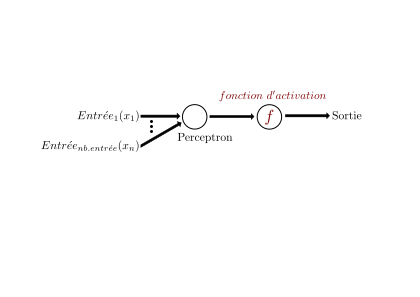
\includegraphics[width=\textwidth]{8-activation.png}
		\caption{Utilisation de la fonction d'activation}
	\end{figure}
\end{frame}


\begin{frame}{II - Fonction d'activation}
	\begin{figure}
		\begin{subfigure}[]{0.3\textwidth}
			\includegraphics[width=90px]{0-Sigmoide.png}
			\caption{Sigmoïde}
		\end{subfigure}
		\begin{subfigure}[]{0.3\textwidth}
			\includegraphics[width=90px]{0-Tanh.png}
			\caption{Tanh}
		\end{subfigure}
		\begin{subfigure}[]{0.3\textwidth}
			\includegraphics[width=90px]{0-ReLU.png}
			\caption{ReLU}
		\end{subfigure}
	\end{figure}
	\begin{block}{}
		\centering
		\begin{tabular}{ l || c | c | }
			Fonction                            & Formule                                          & Dérivée                                    \\ \hline \\
			Sigmoïde (a)                        & $\mathlarger{\frac{1}{1+e^{-x}}}$                & $f(x) \times (1-f(x))$                     \\ \\
			Tangente Hyperbolique (Tanh) (b)    & $\mathlarger{\frac{e^{x}-e^{-x}}{e^{x}+e^{-x}}}$ & $1-f(x)^2$                                 \\ \\
			Unité Linéaire Rectifiée (ReLU) (c) & $max(0, x)$                                      & $ \left\{\begin{array}{ll}
					0 & \mbox{si } x<0 \\
					1 & \mbox{sinon }\end{array}\right.$ \\
		\end{tabular}
	\end{block}
\end{frame}


\begin{frame}{II - Fonction d'activation : Sigmoïde}
	\begin{figure}
		\centering
		\includegraphics[width=250px]{0-Sigmoide.png}
		\caption{Sigmoïde}
	\end{figure}
\end{frame}


\begin{frame}{II - Fonction d'activation : TANH}
	\begin{figure}
		\centering
		\includegraphics[width=250px]{0-Tanh.png}
		\caption{TANH}
	\end{figure}
\end{frame}


\begin{frame}{II - Fonction d'activation : ReLu}
	\begin{figure}
		\centering
		\includegraphics[width=250px]{0-ReLU.png}
		\caption{ReLu}
	\end{figure}
\end{frame}